\chapter{Giới thiệu}
\label{Chapter1}
\graphicspath{{Chapter1/Chapter1Figs}}

% Ngôn ngữ để viết và trình bày báo cáo khóa luận tốt nghiệp, đồ án tốt nghiệp, thực tập tốt nghiệp (sau đây gọi chung là báo cáo) là tiếng Việt hoặc tiếng Anh. 
% Trường hợp chọn ngôn ngữ tiếng Anh để viết và trình bày báo cáo,  sinh viên cần có đơn đề nghị, được cán bộ hướng dẫn (CBHD) đồng ý và nộp cho bộ phận Giáo vụ của Khoa vào thời điểm đăng ký đề tài để xin ý kiến.
% Báo cáo viết và trình bày bằng tiếng Anh phải có bản tóm tắt viết bằng tiếng Việt.


%Tóm tắt luận văn được trình bày nhiều nhất trong 24 trang in trên hai mặt giấy, cỡ chữ Times New Roman 11 của hệ soạn thảo Winword hoặc phần mềm soạn thảo Latex đối với các chuyên ngành thuộc ngành Toán.

%Mật độ chữ bình thường, không được nén hoặc kéo dãn khoảng cách giữa các chữ.
%Chế độ dãn dòng là Exactly 17pt.
%Lề trên, lề dưới, lề trái, lề phải đều là 1.5 cm.
%Các bảng biểu trình bày theo chiều ngang khổ giấy thì đầu bảng là lề trái của trang.
%Tóm tắt luận án phải phản ảnh trung thực kết cấu, bố cục và nội dung của luận án, phải ghi đầy đủ toàn văn kết luận của luận án.
%Mẫu trình bày trang bìa của tóm tắt luận văn (phụ lục 1).

% Với việc bùng nổ dữ liệu trên mạng Internet hiện nay, con người khó có thể nắm bắt được hết tất cả các thông tin.
% Do đó việc tìm kiếm dữ liệu, thông tin phù hợp với nhu cầu của bản thân dần trở nên khó khăn.
% Việc có một hệ thống gợi ý hỗ trợ chúng ta trong việc tìm kiếm thông tin là cực kỳ hữu ích. 
% Một hệ thống gợi ý sản phẩm là một bài toán trong lĩnh vực khai thác dữ liệu và học máy. 
% Hệ thống gợi ý được xây dựng để dự đoán những sản phẩm phù hợp với người dùng, đặc biệt hiện nay 
% việc đưa ra quyết định khi mà có quá nhiều lựa chọn dành cho người dùng là không hề dễ dàng. 
% Điều này dẫn đến vai trò của một hệ thống gợi ý ngày càng quan trọng hơn, 
% không chỉ hỗ trợ người dùng đưa ra quyết định mà còn đóng góp trong việc phát triển doanh nghiệp
%  khi mà việc thu hút khách hàng và nâng cao trải nghiệm người dùng sẽ phù thuộc vào 
% một hệ thống gợi ý sản phẩm hiệu quả. 
% Có rất nhiều lĩnh vực cần xây dựng hệ thống gợi ý có thể kể đến như thương mại điện thử, 
% các nền tàng cung cấp các dịch vụ đa phương tiện (âm thanh, hình ảnh, video, ...), 
% mạng xã hội (Facebook, tweeter, linkedin, ... ).  
% Theo số liệu tổng hợp được thì 75\% phim được thuê trên Netflix - một nền tảng cung cấp video nổi tiếng hiện nay đến từ hệ thống gợi ý; 38\% lượt click từ người dùng GOOGLE cũng đến từ hệ thống gợi ý và Amazon - một nền tảng mua bán trực tuyến mà 35\% sản phẩm được bán thông qua hệ thống gợi ý sản phẩm. 

% Để xây dựng một hệ thống gợi ý sản phẩm ta có các hướng tiếp cận là 


% Một trong những hướng nghiên cứu đang được quan tâm rộng rãi trong lĩnh vực trí tuệ nhân tạo gần đây
% là tạo ra các thuật toán giúp máy tính có thể ``hiểu'' được sở thích của người dùng và gợi ý cho họ
% các nội dung có liên quan. 

Hiện nay, với việc bùng nổ dữ liệu trên mạng Internet, người dùng có cơ hội tiếp cận
nhiều hơn với đa dạng các sản phẩm trên nền tảng số, song song đó,
các nhà cung cấp dịch vụ trên đó cũng có cơ hội tiếp cận với người dùng nhiều hơn. % đó = nền tảng số = internet
Tuy nhiên, người dùng đang gặp nhiều khó khăn khi tìm kiếm những nội dung phù hợp với nhu cầu của họ khi có quá nhiều sự lựa chọn.
Từ khó khăn đó, hệ thống gợi ý được xây dựng để dự đoán cho người dùng những nội dung - hay còn gọi là sản phẩm phù hợp với họ.
Hơn nữa, nó còn đóng vai trò quan trọng trong sự phát triển của các nhà cung cấp dịch vụ - doanh nghiệp,
khi góp phần giúp nâng cao trải nghiệm người dùng cũng như tăng sự thu hút khách hàng. Theo số liệu tổng hợp được, 
38\% lượt click từ người dùng Google đến từ hệ thống gợi ý và 
Amazon - một nền tảng mua bán trực tuyến mà 35\% sản phẩm được bán thông qua hệ thống gợi ý sản phẩm.

Trong lĩnh vực khoa học máy tính, hệ thống gợi ý sản phẩm là một chủ đề 
đang được quan tâm và nghiên cứu từ cộng đồng nghiên cứu khoa học.
Bài toán xây dựng hệ thống gợi ý được phát biểu như sau:
\begin{itemize}
    \item Đầu vào là lịch sử tương tác của người dùng (user) với các sản phẩm (items). 
    (các sản phẩm có thể là: quảng cáo, bộ phim, bài hát, văn bản để đọc, ... tùy thuộc vào lĩnh vực cụ thể).
    \item Yêu cầu máy tính tự động đưa ra các item (không có trong lịch sử) được dự đoán là phù hợp với người dùng.
    Chúng tôi gọi sản phẩm phù hợp với người dùng là sản phẩm được người dùng ``thích''.
\end{itemize}

Tuy nhiên, việc xây dựng một hệ thống gợi ý sản phẩm một cách hiệu quả là không đơn giản.
Đầu tiên, không có một ``lời giải'' chung cho tất cả trường hợp,
mặc dù đa số các lĩnh vực hiện nay đều có thể áp dụng các hệ thống gợi ý, tuy nhiên không phải là tất cả,
ta cần xét đến nhiều yếu tố khác nhau, 
từ đó mới có thể lựa chọn được ``cách'' để xây dựng hệ thống gợi ý phù hợp. % ``cách'' == ``hướng tiếp cận''
Từ thực tế cho thấy, các lĩnh vực mà sản phẩm ``tiêu thụ'' và ``sản xuất'' nhanh như: phim, hình ảnh, âm nhạc, ... 
thì hệ thống gợi ý sẽ ít nhiều đóng vai trò quan trọng. 
Theo số liệu tổng hợp được, một nền tảng cung cấp video nổi tiếng hiện nay - Netflix,
75\% số bộ phim được thuê đến từ hệ thống gợi ý, chứng tỏ sự ảnh hưởng lớn của hệ thống gợi ý đối với lĩnh vực này. 
Mặt khác, hệ thống gợi ý tác động không nhiều đến các lĩnh vực cung cấp dịch vụ hay sản phẩm giá trị cao như:
thuê nhà, phương tiện giao thông, thiết bị điện tử, ... người dùng cần đánh giá thông qua nhiều yếu tố mới có thể quyết định được. 
Thứ hai, tùy thuộc vào nhu cầu của người sử dụng mới có thể lựa chọn ``cách'' mà hệ thống gợi ý hoạt động.
Việc gợi ý các sản phẩm phù hợp với người dùng dựa vào nhóm người dùng có sở thích tương tự với họ 
hay dựa trên tính liên quan đến các sản phẩm họ đã ``thích'' trước đó là khác nhau. 
Điều này cũng liên quan đến khó khăn thứ ba khi xây dựng hệ thống gợi ý, cả trong cộng đồng nghiên cứu khoa học cũng như thực tiễn, 
ta cần một độ đo và một phương pháp để đánh giá một cách tổng thể và khách quan nhất, 
khi mà dữ liệu và các thuật toán để xây dựng hệ thống gợi ý là rất đa dạng.

Để xây dựng hệ thống gợi ý, một hướng tiếp cận chúng ta thường nghĩ ngay đến đầu tiên
là dự đoán các sản phẩm có ``độ tương đồng'' cao so với các sản phẩm người dùng đã ``thích'' trước đó,
hướng tiếp cận này được gọi là ``Content-Based Filtering'' (lọc dựa trên nội dung) (hình~\ref{fig_CBF} mô tả hướng tiếp cận này).
\begin{figure}
    \centering
	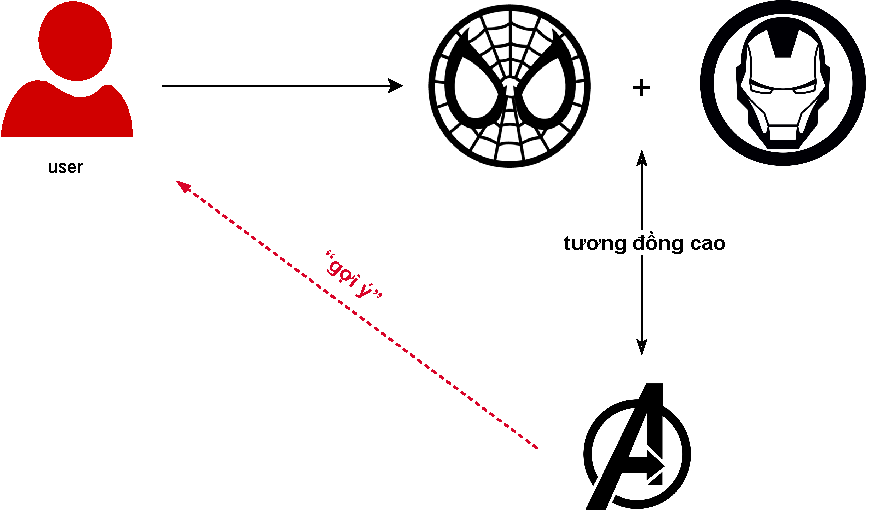
\includegraphics[width=0.6\textwidth]{CBF.pdf}
    \caption{Minh họa cách hoạt động của ``Content-Based Filtering'':
    mô hình gợi ý bộ phim có độ tương đồng cao với các bộ phim
    người dùng đã xem trước đó}
    \label{fig_CBF}
\end{figure}
Với hướng tiếp cận này, mô hình chỉ cần các thuộc tính mô tả của sản phẩm mà 
không đòi hỏi dữ liệu tương tác từ người dùng khác
vì các gợi ý là dành riêng cho từng cá nhân, do đó nó có khả năng nắm bắt tốt các sở thích
đặc biệt của người dùng.
Vì dựa trên tính tương đồng của sản phẩm, hệ thống có thể gợi ý cho người dùng một sản phẩm có ít sự quan tâm từ người dùng khác.
Để áp dụng ``Content-Based Filtering'' cho từng loại dữ liệu cụ thể,
ta cần ``domain knowledge'' cho lĩnh vực đó để thiết kế mô hình.
Trong trường hợp dữ liệu có ít mô tả chi tiết, hướng tiếp cận này vẫn còn hạn chế.

Một hướng tiếp cận khác là tìm ra ``độ tương đồng'' giữa các người dùng với nhau, hay tìm ra được một nhóm người dùng
có cùng sở thích dựa trên dữ liệu tương tác của tất cả người dùng. Khi đó, để có thể gợi ý cho một người dùng cụ thể,
hệ thống sẽ tìm các sản phẩm không có trong lịch sử của người dùng đó, và đã được những người dùng ``tương đồng'' tương tác,
hướng tiếp cận này gọi là ``Collaborative Filtering'' (lọc cộng tác) (hình~\ref{fig_CF} mô tả hướng tiếp cận này).
\begin{figure}
    \centering
    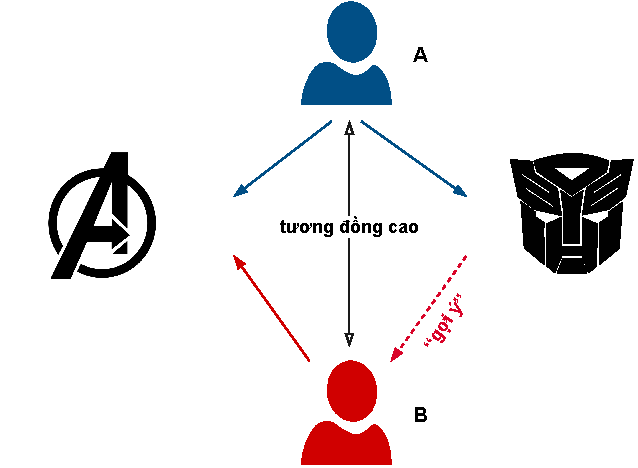
\includegraphics[width=0.6\textwidth]{CF.pdf}
    \caption{Minh họa cách hoạt động của ``Collaborative Filtering'': hai người dùng cùng xem một (hoặc nhiều) bộ phim 
    sẽ được hệ thống đánh giá là hai người dùng ``tương đồng'' nhau, khi đó một bộ phim được
    người dùng A xem sẽ được gợi ý cho người dùng B}
    \label{fig_CF}
\end{figure}
Đối với hướng tiếp cận ``Collaborative Filtering'', mô hình dựa vào lịch sử tương tác từ người dùng khác
và không cần các thuộc tính mô tả của sản phẩm, do đó nó có khả năng tạo ra sự tình cờ cho người dùng:
hệ thống có thể gợi ý một sản phẩm ``tốt'' cho người dùng trong trường hợp sản phẩm đó có ít điểm tương đồng
so với các sản phẩm người dùng đã ``thích'' trước đó. Dữ liệu đầu vào của hướng tiếp cận này là ma trận tương tác
của người dùng và sản phẩm, do đó có thể áp dụng cho nhiều lĩnh vực khác nhau mà không cần thiết kế lại hệ thống.
Tuy nhiên, ``Collaborative Filtering'' có một vấn đề tồn tại là vấn đề khởi động nguội (``cold-start''),
khi một người dùng mới đến với hệ thống thì hệ thống sẽ thường khó đưa ra được gợi ý tốt cho họ,
cũng như khi một sản phẩm được ít người dùng tương tác, hệ thống thường có xu hướng không gợi ý sản phẩm đó.

Ngoài ra, một hướng tiếp cận khác là ``Hybrid'', là sự kết hợp giữa hai hướng tiếp cận bên trên.
Trong giới hạn của luận văn này, chúng tôi chỉ tập trung tìm hiểu về hướng tiếp cận ``Collaborative Filtering'' 
vì hai lý do chính là:
\begin{itemize}
\item ``Collaborative Filtering'' tổng quan hơn so với ``Content-Based Filtering''
- hướng tiếp cận cần ``domain knowledge'' cụ thể để thiết kế hệ thống cho từng lĩnh vực cụ thể
\item Với số lượng lớn cùng sự đa dạng của dữ liệu hiện nay,
ta quan tâm đến sở thích của người dùng nhiều hơn là độ tương đồng giữa các sản phẩm.

\end{itemize}

Việc kết hợp các thông tin chi tiết về người dùng hay từ sản phẩm sẽ là một thông tin hữu ích cho việc xây dựng một hệ thống gợi ý sản phẩm hiệu quả hơn. Nhưng đây là một điều không đơn gảin bởi nó phụ thuộc vào ``domain knowledge'' ở từng lĩnh vực và chúng tôi để lại như một định hướng trong việc nghiên cứu trong tương tai.

Một phương pháp đầu tiên trong việc xây dựng một hệ thống gợi ý sản phẩm theo hướng tiếp cận ``Collaborative Filtering'' trong thuật toán ``Matrix Factorization'' được giới thiệu bởi Hu \cite{MF}, với ý tưởng là xây dựng một mô hình với khả năng ``tái tạo'' lại tương tác của người dùng, trong đó cũng bao gồm các gợi ý cho họ.
Cho đến hiện nay, ``Matrix Factorization'' là một phương pháp đơn giản nhưng vẫn mang lại kết quả tốt.
Tuy nhiên, thuật toán này có các nhược điểm chí mạng mà khó có thể được áp dụng để xây dựng một hệ thống gợi ý sản phẩm quy mô lớn đó là số lượng tham số của mô hình phụ thuộc tuyến tính vào cả số lượng người dùng và số lượng sản phẩm.
Khi mà ngày nay, số lượng người dùng và sản phẩm tăng rất nhanh theo thời gian, ngoài ra sau khi huấn luyện mô hình, mô hình cần thực hiện các bước tối ưu đặc biệt để có thể gợi ý cho người dùng mới. 
Ngoài ra, ``Matrix Factorization'' vẫn còn hạn chế bởi vì nó là một mô hình tuyến tính.
``Asymetric matrix factorization'' là một phương pháp cải tiến từ ``Matrix Factorization'' với ý tưởng là trích xuất đặc trưng của người dùng thông qua các sản phẩm mà họ đã tương tác. Với phương pháp này đã khắc phục được nhược điểm của ``Matrix Factorization'' khi mà sô lượng tham số của người dùng giờ chỉ phụ thuộc vào số lượng sản phẩm có trong hệ thống, khi mà số lượng sản phẩm sẽ tăng chậm hơn rõ rệt so với số lượng người dùng trong hệ thống. Ngoài ra nó cũng giảm bớt chi phí để đưa ra dự đoán cho người dùng mới. Tuy nhiên đây vẫn là một phương pháp tuyến tính do đó mô hình này vẫn chưa thực sự ``mạnh''.
Ở công trình nghiên cứu \cite{AMF} của tác giả Steck đã chỉ ra rằng ``Asymetric Matrix Factorization'' có thể được xem như là một mô hình ``Auto-Encoder'' tuyến tính. ``Auto-Encoder'' là một mô hình học đặc trưng ẩn không giám sát. Mô hình này thường được sử dụng trong những tác vụ như rút trích đặc trưng hay giảm chiều dữ liệu, ... Dựa trên ý tưởng rằng, giả định tương tác của người dùng sẽ được ``phát sinh'' từ một ``đặc trưng ẩn'' là sở thích của họ, và ta sẽ xây dựng một mô hình phát sinh được đặc trưng ẩn của người dùng từ dữ liệu tương tác của người dùng với hệ thống các sản phẩm, sau đó đặc trưng ẩn được sử dụng để đưa ra gợi ý sản phẩm cho người dùng. Với ý tưởng trên, đã có nhiều nghiên cứu để áp dụng mô hình ``Auto-Encoder'' trong bài toán xây dựng hệ thống gợi ý \cite{autorec,cdae,mvae} để có thể tận dụng sức mạnh của các hàm phi tuyến, cụ thể là mạng nơ-ron (là kiến trúc cơ bản của các mô hình được dùng huấn luyện trong lĩnh vực học máy) nhằm giúp có được một mô hình có sức mạnh tốt hơn.
``AutoRec'' \cite{autorec} được Sedhain giới thiệu sử dụng kiến trúc mô hình ``Auto-Encoder'' để đưa ra gợi ý cho người dùng bằng cách huấn luyện mô hình để tái tạo lại dữ liệu tương tác của người dùng sau khi trích xuất đặc trưng ẩn từ dữ liệu tương tác của họ. ``Collaborative denoising auto-encoders for top-n recommender systems'' \cite{cdae} (CDAE) được Wu giới thiệu hướng đến bài toán đưa ra gợi ý là top-N sản phẩm phù hợp với người dùng. Mô hình này dã được xây dựng để phù hợp hơn với bài toán xây dựng hệ thống gợi ý sản phẩm khi mà quan tâm đến việc đưa ra top các sản phẩm phù hợp với người dùng thay vì tái tạo lại tương tác của họ. Ngoài ra, CDAE còn cải tiến từ ``AutoRec'' đó là thêm ``nhiễu'' vào dữ liệu huấn luyện nhằm giúp mô hình tránh được tình trạng ``Overfitting'' (là trình trạng mà mô hình học ``tủ'' trên tập dữ liệu được huấn luyện nên mô hình đạt kết quả thấp trên các tập dữ liệu kiểm định), thường gặp khi huấn luyện mạng nơ-ron với hàm kích hoạt phi tuyến.
Một trong những phương pháp nổi bật nhất tới thời điểm hiện tại trong việc sử dụng kiến trúc mô hình ``Auto-Encoder'' để xây dựng mô hệ thống gợi ý sản phẩm thì ``Variational Autoencoder for Collaborative Filtering''\cite{mvae} được giới thiệu bởi tác giả Liang là một phương pháp sử dụng mô hình ``Variational Auto-encoder'' (VAEs) - một biến thể của mô hình ``Auto-Encoder'' cơ bản để xây dựng một hệ thống gợi ý sản phẩm hiệu quả.
Điểm khác biệt của VAEs so với các phương pháp kể trên đó là đặc trưng ẩn được phát sinh là một phân phối xác suất thay vì là ``một điểm dữ liệu cố định'' (``Auto-Encoder'' và ``Denosing Auto-Encoder'' sẽ nhận dữ liệu đầu vào ở chiều không gian ``cao'' và trích xuất đặc trưng ẩn là một điểm dữ liệu ở chiều không gian ``thấp'' hơn mà vẫn thể thể hiện được ``tính chất'' của dữ liệu ban đầu). Bên cạnh đó, nền tảng của VAEs đó là dựa trên phương pháp ``Variational Inference'', một phương pháp trong lĩnh vực xác suất thống kê được dùng để suy diễn dữ liệu ``ẩn'' dựa trên những dữ liệu ta quan sát được. Đặc điểm của phương pháp này là có thể áp dụng tốt cho dữ liệu thưa, có nghĩa là đối với dữ liệu quan sát được hạn chế thì việc ``suy diễn'' dữ liệu vẫn đạt được kết quả tốt.
Bên cạnh đó, đối với bài toán xây dựng hệ thống gợi ý sản phẩm thì thông thường mỗi người dùng chỉ tương tác với một lượng tỉ lệ nhỏ các sản phẩm so với toàn bộ sản phẩm có trong hệ thống, do đó việc áp dụng phương pháp ``Variational Inference'' hay nói cách khác là VAEs sẽ phù hợp với bài toán xây dựng hệ thống gợi ý sản phẩm dựa trên ý tưởng phát sinh tương tác của người dựa vào đặc trưng ẩn của người dùng. 

Tuy có những lợi điểm trên nhưng trong thực tế thì việc áp dụng VAEs ``hoạt động'' tốt với bài toán xây dựng hệ thống gợi ý sản phẩm thì không dễ.
Để VAEs ``hoạt động'', có hai việc cần phải giải quyết là: (i) kết quả trả về từ mô hình sẽ là tập các sản phẩm được dự đoán là có khả năng cao là phù hợp với người dùng chứ việc tái tạo lại dữ liệu ban đầu không phải mục tiêu chính trong việc xây dựng hệ thống gợi ý sản phẩm và (ii) đánh đổi giữa việc tái tạo lại dữ liệu và việc đặc trưng ẩn được phát sinh tuân theo giả định của ta về phân phối xác suất.
Để kết quả trả về từ mô hình là tập các sản phẩm có ``xác suất'' phù hợp với người dùng thì chúng tôi sử dụng hàm 
% ``Multinomial log-likelihood'' (hàm log-likelihood là hàm số dùng để đánh giá bộ trọng số của mô hình), 
``Multinomial log-likelihood'' (một phương pháp đánh giá bộ tham số của mô hình với giả định dữ liệu tương tác của người dùng tuân theo một phân phối đa thức),
``Multinomial log-likelihood'' sẽ khiến kết quả trả về từ mô hình thể hiện ``giá trị độ lớn về xác suất'' và các sản phẩm sẽ phải ``cạnh tranh'' với nhau để có thể đạt được xác suất được chọn cao hơn (vì kết quả trả về sẽ phải ràng buộc là tổng kết quả trả về sẽ bằng 1 hay xác suất được chọn của các sản phẩm trả về từ mô hình sẽ có tổng bằng 1).
Tuy không được sử dụng nhiều trong lĩnh vực xây dựng hệ thống gợi ý sản phẩm, thay vào đó, ``Multinomial log-likelihood'' lại thường được sử dụng nhiều trong các lĩnh vực về mô hình ngôn ngữ (Language models) hay về các bài toán trong lĩnh vực kinh tế (Ecomomics) nhưng chúng tôi tin rằng ``Multinomial log-likelihood'' sẽ là một lựa chọn phù hợp trong lĩnh vực xây dựng hệ thống gợi ý sản phẩm.
Về vấn đề đánh đổi giữa việc tối thiểu độ lỗi trong việc mô hình hóa dữ liệu và việc đảm bảo đặc trưng ẩn được phát sinh tuân theo phân phối xác suất được giả định thì chúng tôi sử dụng một siêu tham số mới để kiểm soát việc đánh đổi này.
Tuy nhiên, với việc sử dụng siêu tham số để kiểm soát về việc đánh đổi nói trên thì ta sẽ cần phải giải quyết thêm một vấn đề khác đó là việc lựa chọn siêu tham số phù hợp cho mô hình.
Thường thì việc lựa chọn siêu tham số cho các mô hình học là một công đoạn tốn thời gian và phiền phức khi mà ta cần phải chạy mô hình nhiều lần với các siêu tham số khác nhau để chọn ra được siêu tham số để mô hình có kết quả tốt.
Như vậy, có hai câu hỏi được trả lời để mở rộng VAEs cho bài toán xây dựng hệ thống gợi ý sản phẩm là: (i) tại sao Multinomial log-likelihood lại phù hợp hơn với bài toán xây dựng hệ thống gợi ý sản phẩm?; (ii) Làm sao để tối ưu được việc đánh đổi giữa độ lỗi trong việc mô hình hoá dữ liệu và việc đảm bảo đặc trưng ẩn có được từ mô hình được ``chính quy hoá'' theo một phân phối xác suất được giả định. Cụ thể:
\begin{itemize}
    \item Chúng tôi tiến thành thực hiện huấn luyện mô hình VAE với hàm ``Multinomial log-likelihood'' và chúng tôi gọi VAEs với hàm ``Multinomial log-likelihood'' là Mult-VAEs. Bên cạnh đó, chúng tôi cũng thực hiện huấn luyện VAE để so sánh hàm log-likelihood này với các hàm log-likelihood thường được áp dụng khi huấn luyện VAEs là Gaussian log-likelihood và Logistic likelihood.
    \item Hơn nữa, chúng tôi cũng đề xuất một siêu tham số để kiểm soát việc đánh đổi thường gặp khi huấn luyện VAEs. Và phương pháp để lựa chọn siêu tham số này thay vì phải thực hiện huấn luyện với các gía trị siêu tham số khác nhau.
\end{itemize}

Với hai thành phần trên (sử dụng hàm multinomal log-likelighood và siêu tham sô kiểm soát sự đánh đổi trong lúc huấn luyện), kết quả thí nghiệm trên các bộ dữ liệu lớn trong tác vụ xây dựng hệ thống gợi ý sản phẩm như Movielens-20M và Million Song Datasets cho thấy Mult-VAEs đạt được kết quả ấn tượng, ngoài ra việc sử dụng hàm multinomial log-likelihood cho kết quả tốt hơn so với các hàm log-likelihood thông dụng khác.

Phần còn lại của khóa luận được trình bày như sau:
\begin{itemize}
    \item Chương~\ref{Chapter2} trình bày sơ lượt về mô hình ``Auto-Encoder'' và các kiến thức nền tảng của mô hình ``Variational Auto-Encoder''.
    \item Chương~\ref{Chapter3} trình bày về cách áp dụng mô hình ``Variational Auto-Encoder'' cùng với hàm lỗi Multinomial log-likelihood cho bài toán xây dựng hệ thống gợi ý. Bên cạnh đó, chương này cũng phân tích các hạn chế của mô hình đồng thời đề xuất phương pháp giúp giải quyết các hạn chế đó. Chương này là phần chính của khóa luận.
    \item Chương~\ref{Chapter4} trình bày về các thí nghiệm và các kết quả đạt được.
    \item Cuối cùng, kết luận và hướng phát triển được trình bày ở chương~\ref{Chapter5}.
\end{itemize}

